\documentclass[12pt]{book}
\usepackage[width=4.375in, height=7.0in, top=1.0in, papersize={5.5in,8.5in}]{geometry}
\usepackage[pdftex]{graphicx}
\usepackage{amsmath}
\usepackage{amssymb}
\usepackage{tipa}
%\usepackage{txfonts}
\usepackage{textcomp}
%\usepackage{amsthm}
%\usepackage{array}
%\usepackage{xy}
\usepackage{fancyhdr}
\usepackage[brazil]{babel}
\usepackage[utf8]{inputenc}
\usepackage{indentfirst}

%Colocar isso no outro doc e comentar style arduino

\usepackage{listings}
\usepackage{float}
\usepackage{xcolor}

\sloppy

% set the default code style
\lstset{
    frame=tb, % draw a frame at the top and bottom of the code block
    breaklines=true,
    basicstyle=\scriptsize,
    tabsize=4, % tab space width
    showstringspaces=false, % don't mark spaces in strings
    numbers=left, % display line numbers on the left
    commentstyle=\color{green}, % comment color
    keywordstyle=\color{blue}, % keyword color
    stringstyle=\color{red} % string color
}

%%Entnommen aus:
%http://tex.stackexchange.com/questions/211415/how-to-set-up-listings-for-use-code-from-arduino

%%%%%%%%%%%%%%%%%%%%%%%%%%%%%%%%%%%
%%%%%%%%%%%%%%%%%%%%%%%%%%%%%%%%%%%

%Die Umgebung für Arduino-Code wird aufgerufen mit
%\begin{lstlisting}[style=Arduino]
%	...Arduino-Code...
%\end{lstlisting}
%Kleine Überschriften mit
%\minisec{Sketch XY: Leuchte etc}

\usepackage{color}
\usepackage{mwe}
\usepackage{etoolbox} 
%\usepackage{typearea}
\usepackage{listings} 

%%%%Umlaute äöü für dieses Paket definieren
\lstset{basicstyle=\ttfamily}
\lstset{literate=%
  {Ö}{{\"O}}1
  {Ä}{{\"A}}1
  {Ü}{{\"U}}1
  {ß}{{\ss}}2
  {ü}{{\"u}}1
  {ä}{{\"a}}1
  {ö}{{\"o}}1
}
%%%%%%%%%%%%%%%%%%%%%%%%%%%%%%%%%%%%%%%%%%%%   
\usepackage{etoolbox}    

\definecolor{mygreen}{rgb}{0,0.6,0}
\definecolor{mygray}{rgb}{0.47,0.47,0.33}
\definecolor{myorange}{rgb}{0.8,0.4,0}
\definecolor{mywhite}{rgb}{0.98,0.98,0.98}
\definecolor{myblue}{rgb}{0.01,0.61,0.98}
\definecolor{mycoment}{rgb}{0.4,0.5,0.3}

\newcommand*{\FormatDigit}[1]{\ttfamily\textcolor{mygreen}{#1}}
%% http://tex.stackexchange.com/questions/32174/listings-package-how-can-i-format-all-numbers
\lstdefinestyle{FormattedNumber}{%
    literate=*{0}{{\FormatDigit{0}}}{1}%
             {1}{{\FormatDigit{1}}}{1}%
             {2}{{\FormatDigit{2}}}{1}%
             {3}{{\FormatDigit{3}}}{1}%
             {4}{{\FormatDigit{4}}}{1}%
             {5}{{\FormatDigit{5}}}{1}%
             {6}{{\FormatDigit{6}}}{1}%
             {7}{{\FormatDigit{7}}}{1}%
             {8}{{\FormatDigit{8}}}{1}%
             {9}{{\FormatDigit{9}}}{1}%
             {.0}{{\FormatDigit{.0}}}{2}% Following is to ensure that only periods
             {.1}{{\FormatDigit{.1}}}{2}% followed by a digit are changed.
             {.2}{{\FormatDigit{.2}}}{2}%
             {.3}{{\FormatDigit{.3}}}{2}%
             {.4}{{\FormatDigit{.4}}}{2}%
             {.5}{{\FormatDigit{.5}}}{2}%
             {.6}{{\FormatDigit{.6}}}{2}%
             {.7}{{\FormatDigit{.7}}}{2}%
             {.8}{{\FormatDigit{.8}}}{2}%
             {.9}{{\FormatDigit{.9}}}{2}%
             %{,}{{\FormatDigit{,}}{1}% depends if you want the "," in color
             {\ }{{ }}{1}% handle the space
             ,%
}


\lstset{%
  backgroundcolor=\color{mywhite},   
  basicstyle=\footnotesize,       
  breakatwhitespace=false,         
  breaklines=true,                 
  captionpos=b,                   
  commentstyle=\color{mycoment},    
  deletekeywords={...},           
  escapeinside={\%*}{*)},          
  extendedchars=true,              
  %frame=shadowbox,                    
  keepspaces=true,                 
  keywordstyle=\color{myorange},       
  language=Octave,                
  morekeywords={*,...},            
  numbers=left,                    
  numbersep=5pt,                   
  numberstyle=\bfseries\tiny\color{mygray}, 
  rulecolor=\color{black},         
  %rulesepcolor=\color{myblue},
  showspaces=false,                
  showstringspaces=false,          
  showtabs=false,                  
  stepnumber=1,                    
  stringstyle=\color{myorange},    
  tabsize=2,                       
  title=\lstname,
  emphstyle=\bfseries\color{blue},%  style for emph={} 
}    

%% language specific settings:
\lstdefinestyle{Arduino}{%
    style=FormattedNumber,
    keywords={void},%                 define keywords
    morecomment=[l]{//},%             treat // as comments
    morecomment=[s]{/*}{*/},%         define /* ... */ comments
    emph={HIGH, OUTPUT, LOW},%        keywords to emphasize
}

\newtoggle{InString}{}% Keep track of if we are within a string
\togglefalse{InString}% Assume not initally in string


%colocar aqui os capitulos da apostila

\pagestyle{fancy}
\renewcommand{\chaptermark}[1]{\markboth{#1}{}}
\renewcommand{\sectionmark}[1]{\markright{\thesection\ #1}}
\fancyhf{}
\fancyhead[LE,RO]{\bfseries\thepage}
\fancyhead[LO]{\bfseries\rightmark}
\fancyhead[RE]{\bfseries\leftmark}
\renewcommand{\headrulewidth}{0.5pt}
\renewcommand{\footrulewidth}{0pt}
\addtolength{\headheight}{0.5pt}
\setlength{\footskip}{0in}
\renewcommand{\footruleskip}{0pt}
\fancypagestyle{plain}{%
\fancyhead{}
\renewcommand{\headrulewidth}{0pt}
}
%
%\parindent 0in
\parskip 0.05in
%
\begin{document}
\frontmatter
%
\chapter*{\Huge \center Internet das Coisas }
\thispagestyle{empty}
%{\hspace{0.25in} \includegraphics{./ru_sun.jpg} }
\section*{\center Cloadoaldo Basaglia da Fonseca \\Douglas Lohmann \\Marco Aurélio Graciotto Silva \\Paulo Cesar Gonçalves}
\newpage

% licensa / direitos autorais
\subsection*{\center \normalsize Este trabalho está licenciado sob uma Licença Creative Commons Atribuição 4.0 Internacional. Para ver uma cópia desta licença, visite \\ http://creativecommons.org/licenses/by/4.0/.}

\subsection*{\center \normalsize Os diagramas de projeto foram construídos com o software Fritzing e estão licenciados sob uma Licença Creative Commons Atribuição 4.0 Internacional}

\subsection*{\center \normalsize Este trabalho foi financiado pela Fundação Araucária - Apoio ao Desenvolvimento Científico e Tecnológico do Paraná, por meio do Edital Redes Digitais de Cidadania do Estado do Paraná (Ministério das Comunicações), aprovado em 2013. Foi desenvolvido por alunos e professores da  Universidade Tecnológica Federal do Paraná (UTFPR), campus Campo Mourão}

\subsection*{\center \normalsize Uma versão online desse material está disponível em https://github.com/lohmanndouglas/Iot-Compute-Voce-Mesmo.git }


%

% dedicatoria 
%\chapter*{\center \normalsize To my Son}
%
\tableofcontents
%
\mainmatter

% Objetivos 
\chapter{Uma Visão Geral}
% your text here
Computadores pessoais e smartphones formam uma rede de dispositivos conectados a Internet. A questão agora é permitir  que outros dispositivos tais como relógios, máquinas de lavar, geladeiras e demais objetos do nosso cotidiano possam conectar-se a rede e trocar informações. Esta fase em formação está introduzindo um novo paradigma chamado de Internet das Coisas (do inglês, Internet of Things - IoT), no qual pessoas, animais e coisas do nosso cotidiano estão conectados à rede e interagirem entre si.


A Internet das Coisas mudará tudo, inclusive nós mesmos. Considerando o impacto que Internet já causou na comunicação, nos negócios, na ciência, no governo e na educação, percebemos claramente que a Internet é uma das mais importantes e poderosas invenções de toda a história humana \cite{daveevans2011}. Devido ao desenvolvimento das tecnologias de informação, principalmente da Internet, podemos nos comunicar tranquilamente com qualquer parte do mundo, Desta forma, possuímos a oportunidade de conhecer muitas coisas - novas pessoas, culturas, sistemas políticos, desenvolvimento de cada país e muitas coisas mais - por meio de alguns cliques. 


Podemos dividir a Internet em três fases. A primeira fase é a Internet como uma rede de computadores. Na segunda fase, a Internet pode ser considerada uma rede de pessoas e comunidades e atualmente estamos vivendo a evolução para terceira fase, a Internet das Coisas (IoT). Nesta fase a rede passa a interligar vários tipos de objetos e dispositivos inteligentes do nosso cotidiano que vão interagir entre si e conosco \cite{nicbr}.
Segundo \cite{atzori2010internet}, a ideia básica de IoT consiste na presença de uma diversidade de  objetos que interagem e cooperam entre si a fim de atingir um objetivo comum. Para tal compartilham informações utilizando métodos de endereçamento único e protocolos de comunicação padronizados. 

Este material apresenta os principais conceitos relacionados a Internet das Coisas e também apresenta uma atividade prática para implementação de IoT. Os próximos tópicos são referências básicas para a construção da rede de sensores e a comunicação dos sensores com a Internet. 

%
\chapter{Materiais e Softwares Utilizados} \label{MateSof}

Este capítulo apresenta uma breve descrição dos principais materiais e softwares necessários para implementação dos projetos propostos.  

\section{Arduino}

Arduino~\footnote{https://www.arduino.cc/en/Guide/Introduction} é uma plataforma de prototipagem de código aberto baseada na fácil utilização do software e hardware. As placas Arduino são capazes de efetuarem leitura de uma entrada (sensores) e transformar em uma de saída (Atuadores). O projeto Arduino nasceu no Ivrea Interaction Design Institute como uma ferramenta fácil para prototipagem rápida, destinado a estudantes sem conhecimento aprofundado em eletrônica e programação. 

A plataforma Arduino possui uma IDE para a programação e para gravar códigos na placa, a IDE possui ainda suporte a Linux, Mac e Windows. 

Existem diversas placas de hardware Arduino, sendo a mais comum a Arduino Uno. As placas diferem basicamente no microcontrolador embutido, no número de entradas/saídas, na frequência de processamento e entre outras configurações.

Neste Material vamos utilizar o Arduino Uno por ser facilmente encontrado no mercado e apresentar baixo custo de aquisição se comparado com outras plataformas de hardware.

A conexão de novos componentes no Arduino é possível por meio de placas de expansão (\textit{shields}), essa placas aumentam as funcionalidades do Arduino. Os \textit{shields} mais conhecidos são os \textit{shields} para controle de motores~\footnote{https://www.arduino.cc/en/Main/ArduinoMotorShieldR3} e o Ethernet para comunicação do Arduino com a Internet, como o da Figura~\ref{fig:motorControl}.  

\begin{figure}[ht]
      \centering
      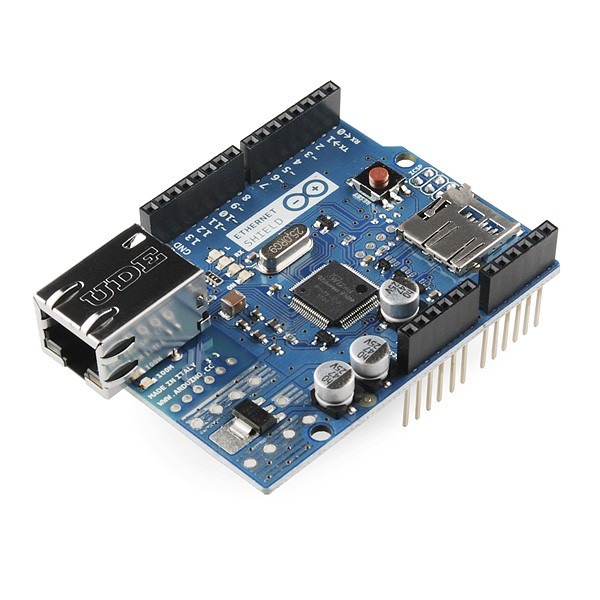
\includegraphics[scale=0.35]{figuras/image_321.jpg}
      \caption{Shield para controle de motores}
      \label{fig:motorControl}
\end{figure}

A comunicação do Arduino com \textit{shields} é realizada pelo protocolo Serial Peripheral Interface (SPI)~\footnote{https://www.arduino.cc/en/Reference/SPI
}  , ele é um protocolo de dados seriais síncronos utilizado em microcontroladores para comunicação entre o microcontrolador e um ou mais periféricos, sendo que também pode ser utilizado entre dois microcontroladores.

A comunicação SPI sempre tem um master. Isto é, sempre um será o master e o restante será slave. Por exemplo, o Arduino é o master e os outros periféricos são slaves. Esta comunicação contém 4 conexões:

\begin{itemize}
  \item MISO (Master IN Slave OUT) - Dados do Slave para Master;
  \item MOSI (Master OUT Slave IN) - Dados do Master para Slave;
  \item SCK (Serial Clock) - Clock de sincronização para transmissão de dados entre o Master e Slave;
  \item SS (Slave Select) - Seleciona qual Slave receberá os dados.
\end{itemize}

\subsection{Arduino IDE}

Para programação no arduino, utiliza-se a linguagem Wiring. O ambiente de programação oferece recursos que facilitam a criação de aplicações e sua gravação no dispositivo.

Os projetos (Sketches) são escritos na linguagem Wiring e salvos com a extensão .ino, possuindo a seguinte estrutura:

\lstinputlisting[language=C++, caption={Estrutura código Arduino}]{code/arduino.ino}

A função setup() é o código de inicialização dos componentes, enquanto a função loop é o laço principal do programa, que contém o código que será executado repetidamente.

\subsection{Arduino Uno}

O Arduino Uno~\footnote{https://www.arduino.cc/en/Main/ArduinoBoardUno} opera com uma velocidade de clock de 16 MHz, possui 14 pinos de entrada e saída digitais e 6 pinos de entrada e saída analógica, memória flash de 32 KB (0.5 KB usados pelo Bootloader), memória SRAM de 2 KB e 1 KB de memória EEPROM. 

A placa pode ser alimentada pela conexão USB ou por uma fonte de alimentação externa. Para alimentação externa é utilizado um conector Jack com positivo no centro, sendo que a placa suporta alimentação de 6 à 20 volts. Porém, é recomendado que a fonte de alimentação externa possua tensão entre 7 e 12 volts. 

A Figura~\ref{fig:arduino} ilustra o Arduino Uno utilizado neste projeto, ele tem 14 pinos de entradas/saídas digitais. Alguns desses pinos possuem funções especificas como PWM (pinos 3, 5, 6, 9, 10 e 11 ), comunicação serial (pinos 0 e 1) e interrupção externa (pinos 2 e 3).
Para interface com o mundo analógico, a placa Arduino UNO possui 6 entradas, onde cada uma tem a resolução de 10 bits.

\begin{figure}[ht]
      \centering
      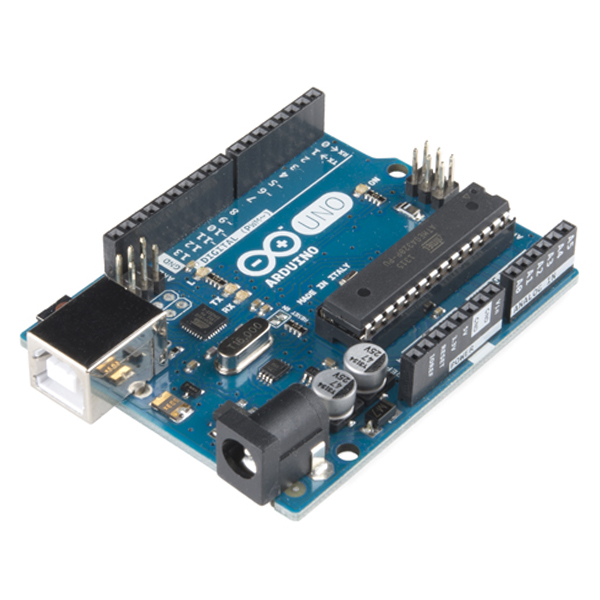
\includegraphics[scale=0.35]{figuras/arduino.jpg}
      \caption{Arduino Uno}
      \label{fig:arduino}
\end{figure}



\section{Radio RF - nRF24l01}

Nesta apostila vamos utilizar o módulo de rádio frequência nRF24l01~\footnote{http://www.nordicsemi.com/eng/Products/2.4GHz-RF/nRF24L01} fabricado pela Nordic, este módulo trabalha na frequência de 2.4 GHz.

A conexão é realizada por um conector de 8 pinos muito próximos uns dos outros, o que impossibilita a conexão direta do módulo com a protoboard, sendo assim, a conexão com o módulo pode ser feita com jumpers macho-fêmea e outra possibilidade é construir um shield para adaptação, para que o nRF24l01 encaixe na protoboard.

O alcance do módulo varia de 10 metros em ambiente fechado à 50 metros em ambiente aberto. Uma outra vantagem é que um mesmo módulo pode atuar como emissor ou receptor, apenas realizando-se uma configuração por software. Sua tensão de alimentação é de 1,9 à 3.6V, e os pinos de sinal podem trabalhar normalmente com nível de sinal de 5V. 

Existe uma versão do módulo com antena externa, essa versão possibilita distância maior de comunicação entre os módulos, porém tem preço maior e não é tão compacto quanto o módulo com antena embutida. 

\begin{figure}[ht]
      \centering
      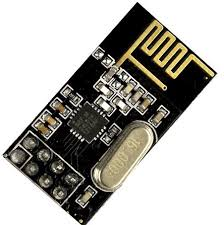
\includegraphics[scale=0.30]{figuras/nrf24l01.jpg}
      \caption{Rádio nRF24L01}
      \label{fig:nRF24L01}
\end{figure}



\section{Sensores e Atuadores}

Esta seção é uma breve descrição dos principais sensores e atuadores utilizados para realizar os projetos propostos nesse material.  

\subsection{DTH11}

O DTH11~\footnote{https://learn.adafruit.com/dht} é um sensor de baixo custo para a medição de temperatura e umidade do ambiente. Sua faixa de medição de temperatura vai de 0° a 50° Celsius, com 2\% de margem de erro. Já a medição de umidade pode variar de 20\% até 90\% com precisão de 5\%.

O sensor possui 4 pinos: um pino para o GND(ground), um para a alimentação(5V), um pino para envio dos dados que é conectado a uma entrada digital do Arduino e um pino que não é utilizado.

\begin{figure}[ht]
      \centering
      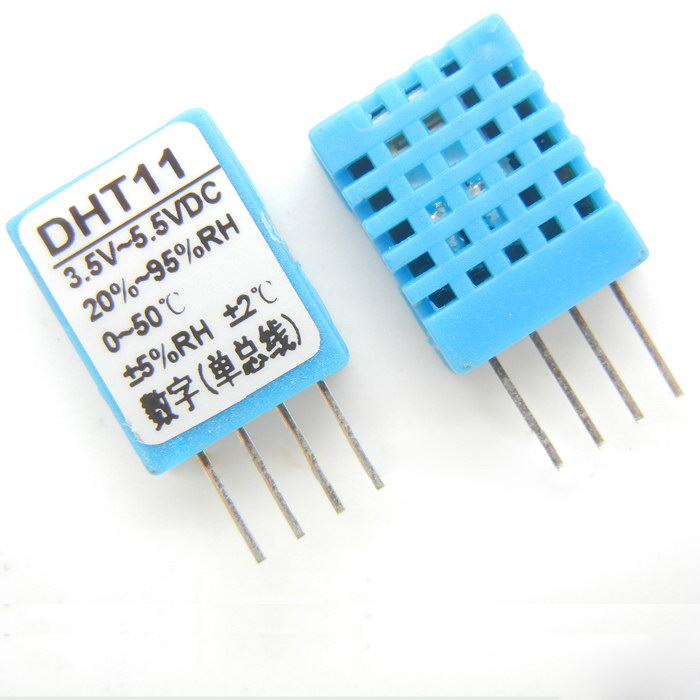
\includegraphics[scale=0.20]{figuras/FDHT11.jpg}
      \caption{Sensor DTH11}
      \label{fig:Sdth11}
\end{figure}

\subsection{LDR}

O LDR (do inglês, Light Dependent Resistor), ou Resistor dependente de Luz, é uma fotorresistência, ou seja, um resistor cuja resistência varia de acordo com a intensidade da luz que incidir sobre ele. 

Utilizando um multímetro pode-se medir a resistência de um LDR quando exposto a uma determinada intensidade de luz. Basicamente, um LDR vai ter sua resistência máxima quando estiver em completa escuridão e mínima quando uma luz muito brilhante estiver incindindo sobre ele.

\begin{figure}[H]
      \centering
      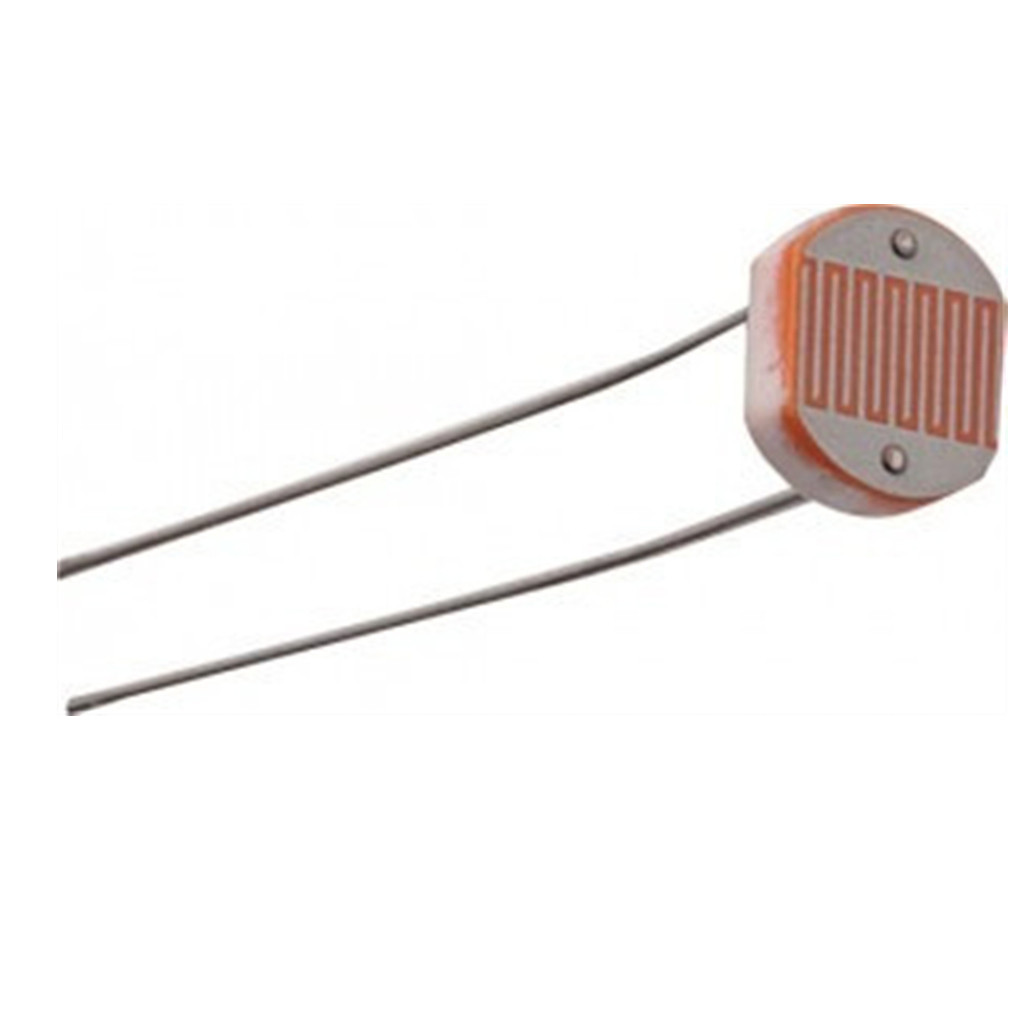
\includegraphics[scale=0.10]{figuras/Fldr.jpg}
      \caption{Sensor LDR}
      \label{fig:SLDR}
\end{figure}



%[https://en.wikipedia.org/wiki/Photoresistor]

\subsection{Relé}

O relé é um dispositivo eletromecânico capaz de desligar ou ligar outros dispositivos. Basicamente, o relé é acionado quando uma corrente elétrica passa a percorrer as espiras da bobina do mesmo, criando assim um campo magnético que atrai ou repele uma alavanca responsável por ativar ou desligar o outro componente ligado ao relé. 

\begin{figure}[ht]
      \centering
      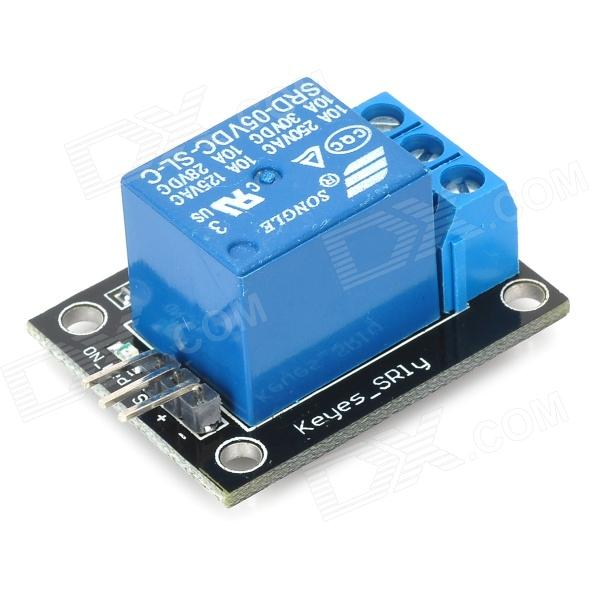
\includegraphics[scale=0.25]{figuras/Frele.jpg}
      \caption{Atuador relé}
      \label{fig:Arele}
\end{figure}

% incluir exemplo de uso

\subsection{Sensor de Movimento (PIR)}

O sensor de movimento (PIR)~\footnote{https://learn.adafruit.com/pir-passive-infrared-proximity-motion-sensor/}é, basicamente, feito de um material piroelétrico, ou seja, seu potencial elétrico varia de acordo com a temperatura, tornando-o capaz de detectar alguns níveis de radiação infravermelha. Ele é construído em duas metades e as duas são conectadas de forma que a diferença de potencial entre elas seja interpretada como um nível alto ou baixo, fazendo assim a detecção de movimento.

\begin{figure}[ht]
      \centering
      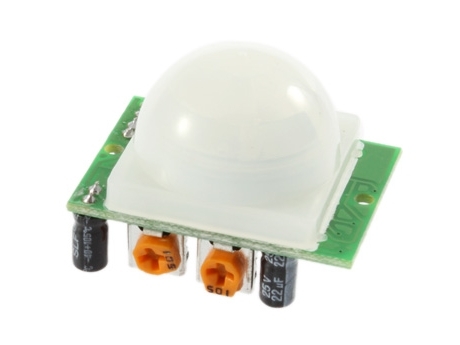
\includegraphics[scale=1.20]{figuras/Fpir.png}
      \caption{Sensor de Movimento PIR}
      \label{fig:SPIR}
\end{figure}

% explicar porque funciona p/ detectar movimento


\subsection{LED}

Light Emitting Diode (LED) ou diodo emissor de luz, é utilizado para emissão de luz em locais onde lâmpadas não são viáveis, por exemplo em produtos da microeletrônica, como sinais de avisos. Existem também LEDs de tamanhos maiores, como os utilizados em sinais de trânsito.

Uma característica marcante do LED diz respeito ao seu baixo consumo de energia, sendo uma alternativa viável para iluminação de ambientes. Outra característica importante é que sua durabilidade é maior que as outras formas de emissão de luz presentes no mercado.

Na maioria dos projetos vamos utilizar o LED como atuador para emitir sinais de aviso. Mais detalhes sobre o funcionamento do LED estão disponíveis em http:\/\/electronics.howstuffworks.com\/led.htm

% [https://en.wikipedia.org/wiki/Light-emitting_diode]
% [http://electronics.howstuffworks.com/led.htm]

\begin{figure}[ht]
      \centering
      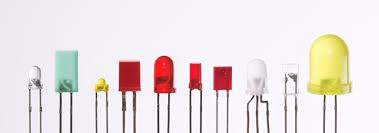
\includegraphics[scale=0.50]{figuras/Fled.jpg}
      \caption{LEDs}
      \label{fig:Aled}
\end{figure}


\section{Protoboard}

A Protoboard é uma placa com uma matriz de furos e conexões condutoras utilizadas para a prototipação de circuitos eletrônicos.

\begin{figure}[ht]
      \centering
      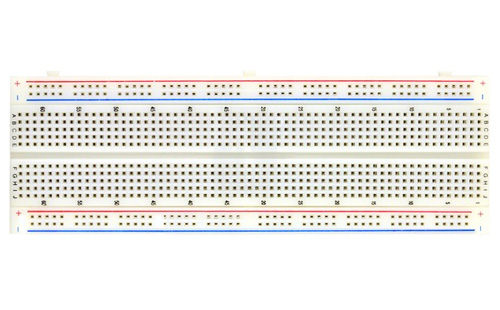
\includegraphics[scale=0.50]{figuras/FProtoboard_2_M.jpg}
      \caption{Protoboard}
      \label{fig:protoboard}
\end{figure}

A Figura~\ref{fig:protoboard} ilustra uma protoboard. Essa placa tipicamente possui trilhas conectadas na vertical que possibilitam a ligação entre componentes e trilhas isoladas na horizontal. 

\section{Conexão de todas as partes}

Para conectar os sensores e atuadores à placa do Arduino, é utilizado cabo jumper. Pode ser encontrado em 3 combinações: macho-macho, macho-fêmea e fêmea-fêmea.

A Figura~\ref{fig:Jmacho} representa jumpers macho. 

\begin{figure}[H]
      \centering
      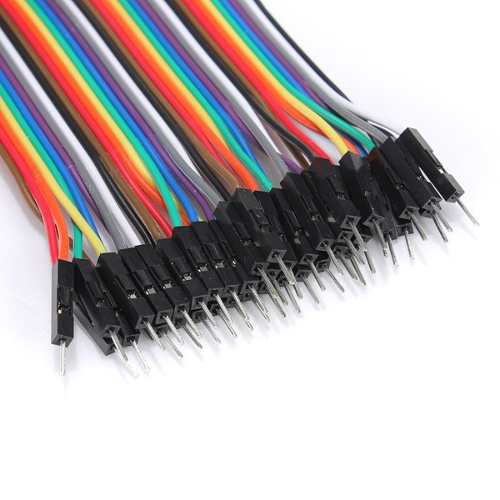
\includegraphics[scale=0.25]{figuras/jumperMachoo.jpg}
      \caption{Jumper Macho}
      \label{fig:Jmacho}
\end{figure}

A Figura~\ref{fig:Jfemea} representa jumpers fêmea.

\begin{figure}[H]
      \centering
      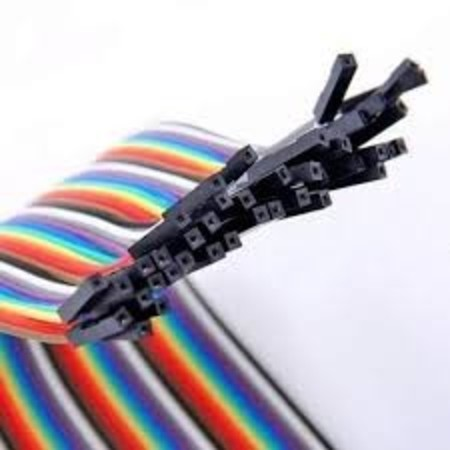
\includegraphics[scale=0.30]{figuras/Jfemea.jpg}
      \caption{Jumper Fêmea}
      \label{fig:Jfemea}
\end{figure}

%explicar/foto macho-macho, macho-femea e femea-femea

\section{Conectando o Arduino ao Rádio}

O rádio nRF24l01+ se comunica com Arduino via interface SPI. O rádio deve ser alimentado com uma tensão de 3.3 volts. 

Como o rádio possui conector de 8 pinos, não é possível conectá-lo a protoboard. Então, devemos utilizar conectores macho-fêmea, como ilustra a Figura~\ref{fig:gat}, para fazer ligação ou construir um shield para adaptação do módulo.

\begin{figure}[H]
      \centering
      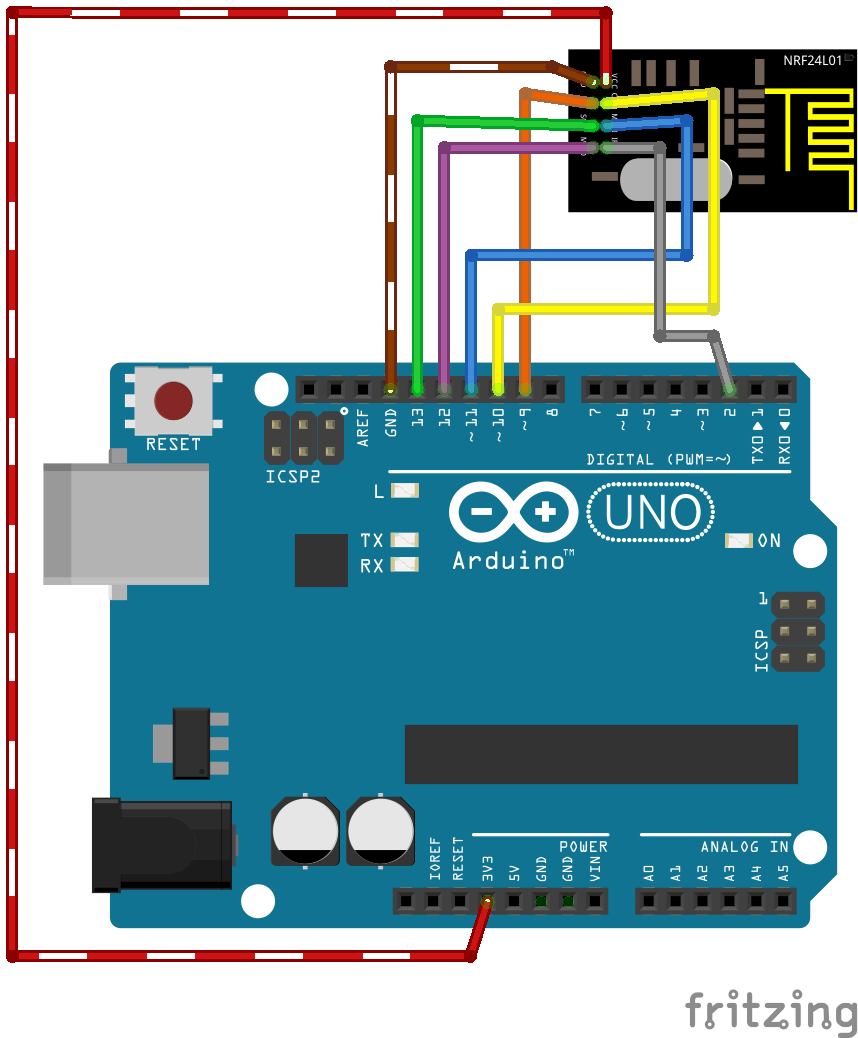
\includegraphics[scale=0.50]{figuras/gateway.png}
      \caption{Conexão rádio e Arduino Uno}
      \label{fig:gat}
\end{figure}

\section{Biblioteca Mysensors}

Mysensors~\footnote{http://www.mysensors.org/} é uma API que fornece um conjunto de protocolos e rotinas para comunicação entre o Arduino, o Rádio transmissor e sensores. 
Com esta biblioteca é possível criar uma abstração de algumas camadas de hardware e software evitando que o usuário tenha que implementar rotinas de baixo nível e protocolos para realizar a comunicação entre o Arduino e Módulo de rádio frequência. A biblioteca fornece códigos de exemplos e uma estrutura de rede já implementada para Internet das Coisas. 

\subsection{Aplicações da biblioteca MySensors}

A biblioteca MySensors fornece uma infinidade de projetos com exemplos de sensores e atuadores já implementados. Algumas possibilidades de aplicação da biblioteca são:

\begin{itemize}
    \item Pequenas automações residenciais, tais como um portão de garagem automático que abre quando um carro se aproxima da entrada ou quando ativado pelo seu \textit{smartphone}; 

    \item Coletar a umidade do ambiente dentro da casa para controlar a ventilação;

    \item Criar uma fechadura inteligente para um determinado cômodo ou armário; 
    
    \item Criar um dispositivo que avisa através de uma mensagem em seu \textit{smartphone} quando a temperatura do frezzer subir caso alguém tenha deixado a porta aberta;

    \item Criar uma identificação única para seu cachorro para que somente ele possa entrar em sua casa.
\end{itemize}

\subsection{Instalar Mysensors}

MySensors é uma biblioteca que funciona integrada com a API do Arduino, para instalação basta adicioná-la a pasta \textit{libraries} do Arduino IDE.





%
\chapter{Infraestrutura da Internet das Coisas}


\section{Componentes envolvidos}

\subsection{O cérebro}

O Arduino foi a escolha para esse projeto, pois tem consumo de energia baixo, é fácil de programar,muitas bibliotecas já estão implementadas e são livres para uso, além disso, é um hardware livre. 

Apesar de não ter um poder computacional muito alto, o Arduino é ideal para uso nesse projeto. Além disso, ele tem pinos (22 no total) que são ideais para conectar sensores e botões. Outra característica é que o Arduino não possui sistema operacional.

\subsection{O rádio}

Com a necessidade de comunicação e coleta de dados dos sensores e devido a possível distância entre eles, é necessário uma conexão sem fio. Para tais fins, é utilizado um pequeno rádio, nesse caso, o modelo nRF24l01, que tem baixo consumo de bateria e baixo preço.

\subsection{Software}

Além dos componentes de hardware, vamos utilizar alguns softwares, na maior parte bibliotecas com alguns exemplos de sensores já implementados. 

\section{Construção da Rede de Sensores e Atuadores}

Utilizando a biblioteca e as plataformas descritas no Capítulo~\ref{MateSof}, é possível configurar uma infraestrutura para a rede IoT, como ilustra a \ref{fig:iot}. A rede implementada possui
basicamente três componentes:
controlador, gateway e nós finais, que são nós sensores e atuadores. Os nós sensores e atuadores são responsáveis
pela interação com o ambiente, seja pela coleta de informações por meio de sensores, emissão de sinais de alerta ou ativação de certos dispositivos por meio de atuadores, por
exemplo, o ar condicionado ou uma lâmpada.

Os principais componentes de uma rede de sensores são apresentados nas próximas subseções.

\begin{figure}[H]
      \centering
      \includegraphics[scale=0.50]{figuras/Diagrama.png}
      \caption{Infraestrutura iot}
      \label{fig:iot}
\end{figure}

A Figura~\ref{fig:iot} ilustra a infraestrutura de uma rede de sensores e atuadores, pode-se perceber a presença do nó gateway conectando os nós sensores e o controlador. Embora na imagem a ligação entre os dispositivos é representada por linhas, na prática a ligação entre os nós na maioria das vezes não é feita por jumper e sim via rádio frequência. 

\subsection{Nó sensor ou atuador}
	Esse nó realiza a leitura de sensores e pode também funcionar como um nó atuador, enviando e recebendo dados do gateway. Esse nó pode funcionar em modo Sleep para economizar bateria.

\subsection{Nó repetidor}
	Esse nó só é necessário quando os nós sensores e gateway não conseguem se comunicar, devido à distância em que estão localizados, por esse motivo não está representado na Figura~\ref{fig:iot}. Esse nó tem como função repetir as dados para outros nós a fim de aumentar a distância de comunicação entre os nós. Em muitas aplicações esse nó não está presente.

\subsection{Nó gateway}

O gateway atua na ligação entre o controlador e rede de rádios. Ele traduz as mensagens do rádio para um protocolo que pode ser entendido por um controlador. 

Na biblioteca MySensors existem três implementações de Gateway: Ethernet Gateway, SerialGateway e MQTTGateway. Nesse material, vamos utilizar o SerialGateway pela facilidade de implementação e, também, pela compatibilidade com o controlador escolhido.
	
\subsection{Controlador}

O controlador pode realizar as seguintes funções:
\begin{itemize}
    \item Enviar parâmetros de configuração para os sensores na rede de rádio (tempo e identificadores de sensores únicos);
    \item Acompanhar os dados mais recentes enviados pelos sensores e atuadores;
    \item Fornecer informações de status de volta para sensores e atuadores, por exemplo, o estado atual (on / off / loadLevel) para uma luz;
    \item Fornecer controles de interface do usuário para atuadores;
    \item Executar horários predefinidos ou cenas, por exemplo, ao pôr do sol acender as luzes do jardim.
\end{itemize}
    
Neste material, vamos utilizar como controlador o Raspberry e o framework Pimatic.

\section{Entendendo o protocolo serial MySensors versão 1.5}

O protocolo utilizado para comunicação entre o serial gateway e controlador consiste de mensagens textuais em que cada dado é separado por ponto e virgula (;) e quebra de linha no final da mensagem. Sendo assim, a mensagem possui a seguinte estrutura:

%colocar uma caixa/imagem

 \vbox{
\noindent \rule{11.1cm}{0.4pt}\par
\noindent node-id; child-sensor-id; message-type; ack; sub-type; payload;\par%\vspace{-0.66\baselineskip}
\noindent \rule[0.90\baselineskip]{11.1cm}{0.6pt}
}



\begin{description}
  \item[node-id] identificação exclusiva do nó que envia ou deve receber a mensagem (endereço);
  \item[child-sensor-id] Cada nó pode ter vários sensores ligados, esse campo identifica qual é o sensor “child” do nó;
  \item[message-type] Tipo de mensagem enviada.
  \item[ack] Outgoing: 0 = mensagem não reconhecida, 1 = pedido ack do nó de destino; Incoming: 0 = mensagem normal, 1 = esta é uma mensagem de ack;
  \item[sub-type] Dependendo da messageType, este campo tem um significado diferente.
  \item[payload] Carga útil (max 25 bytes).
  
\end{description}

\section{Códigos Mysensors}

Nesta seção é apresentado um exemplo de código da biblioteca MySensors. Esse código apresenta os principais métodos utilizados na maioria dos exemplos. 

\lstinputlisting[language=, caption={Código Mysensors}]{code/exemplo.ino}

%colocar srccode{} nas funções 

Para iniciar, precisamos criar uma instância da biblioteca MySensors e depois ativá-la com a instrução gw.begin(). Na primeira vez que o nó é ligado, o controlador atribui um id único a ele. Esse id é salvo na memória EEPROM do Arduino. Caso ele seja religado ou resetado, o id é automaticamente resgatado. O sensor deve ser apresentado para o controlador. Para isso, é utilizado a função gw.present(child-sensor-id, sensor-type).

Para enviar uma mensagem deve-se criar um container MyMessage usando a função msg(child-sensor-id, variable-type). No escopo da função loop, a mensagem é enviada com o método send(msg.set(payload)).

\section{Controlador Pimatic}

Para as atividades desenvolvidas nesse material utilizamos o 
controlador Pimatic. 

Pimatic~\footnote{http://www.mysensors.org/controller/pimatic} é um framework de automação residencial que é executado no Node.js. Ele fornece uma plataforma extensível comum para controle de casa e tarefas de automação
\cite{pimatic}.

A configuração do Pimatic é realizada por meio de somente um arquivo, denominado config.json. Esse arquivo está no formato JSON e é dividido em quatro seções: Configurações (settings), Plugins, Dispositivos (devices) e Regras (Rules). A seguir, exemplos das quatro seções são apresentados.




%
\chapter{Projeto A}

Quando começamos aprender uma nova linguagem, geralmente iniciamos com o exemplo mais básico, o \textit{"Hello Word"}. Nesse primeiro projeto, também vamos começar com a construção do \textit{"Hello Word"} da biblioteca MySensors e Pimatic, monitorando apenas a temperatura e umidade com um único nó sensor. Neste projeto, vamos construir um nó sensor simples com o intuito de monitorar a temperatura e umidade de uma sala. 

\section{Materiais}

Para esse projeto vamos o utilizar os seguintes materiais:
\begin{itemize}
\item 2 Arduinos;
\item Sensor de temperatura e umidade DTH11;
\item 2 Rádios RF;
\item Jumpers.
\end{itemize}

Para obter mais informações sobre os materiais consulte o capítulo ~\ref{MateSof}.

\section{Implementação}

Para a implementação desta atividade é necessário a construção dos seguintes nós.

\subsection{Gateway}

\vbox{
\indent \rule{10.4cm}{0.6pt}\par
\textbf{Esquemático}\par%\vspace{-0.66\baselineskip}
\rule[0.90\baselineskip]{10.4cm}{0.6pt}
}

\begin{figure}[ht]
      \centering
      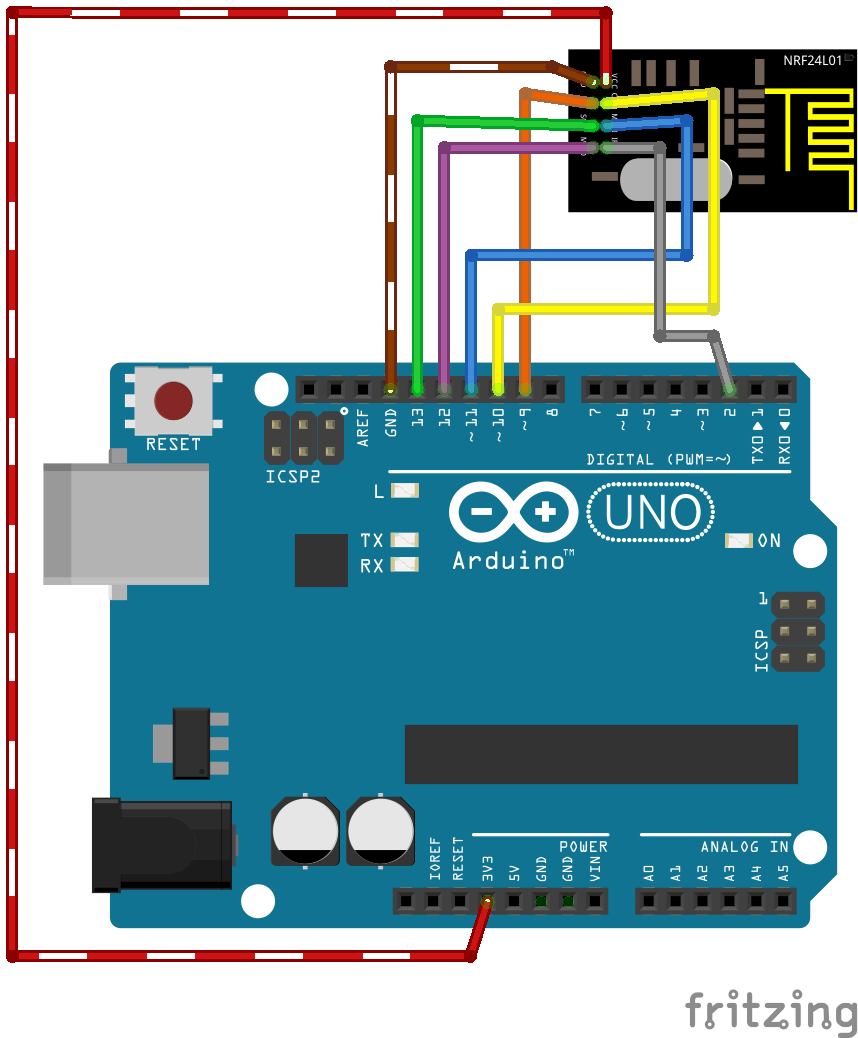
\includegraphics[scale=0.70]{figuras/gateway.png}
      \caption{Gateway}
      \label{fig:gateway}
\end{figure}
\pagebreak
\vbox{
\indent \rule{10.4cm}{0.6pt}\par
\textbf{Código}\par%\vspace{-0.66\baselineskip}
\rule[0.90\baselineskip]{10.4cm}{0.6pt}
}

\lstinputlisting[language=C++, caption={Gateway}]{code/teste.ino}

\subsection{Nó com sensor DTH11}

\vbox{
\indent \rule{10.4cm}{0.6pt}\par
\textbf{Esquemático}\par%\vspace{-0.66\baselineskip}
\rule[0.90\baselineskip]{10.4cm}{0.6pt}
}

\begin{figure}[ht]
      \centering
      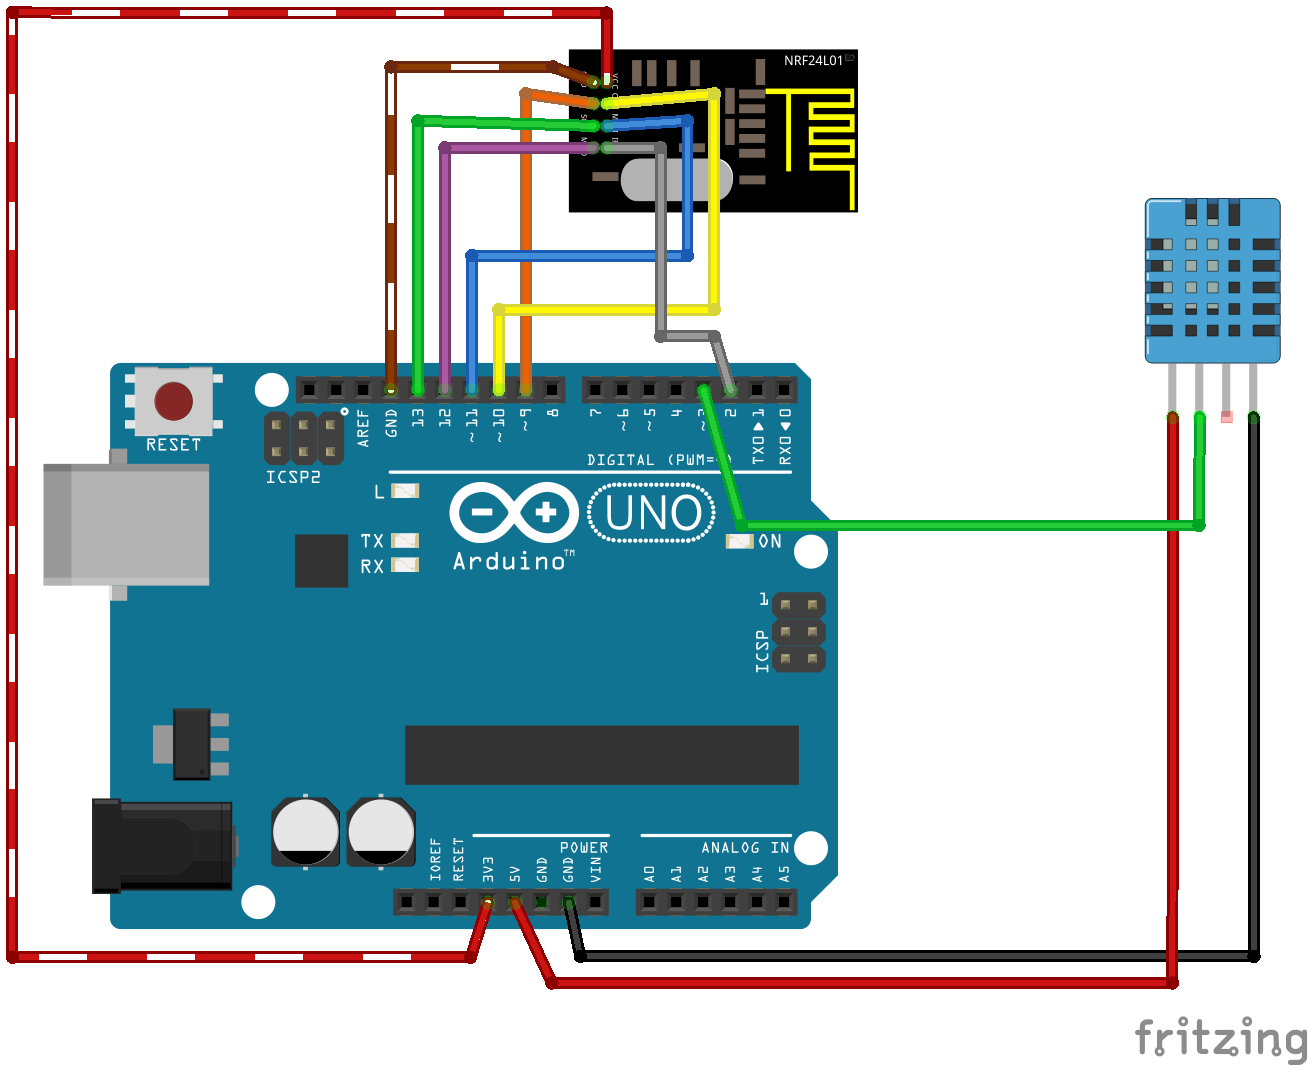
\includegraphics[scale=0.70]{figuras/DTH11_bb.png}
      \caption{Sensor DTH11}
      \label{fig:dth11}
\end{figure}
\pagebreak

\vbox{
\indent \rule{10.4cm}{0.6pt}\par
\textbf{Código}\par%\vspace{-0.66\baselineskip}
\rule[0.90\baselineskip]{10.4cm}{0.6pt}

}

\lstinputlisting[language=C++, caption={dth11}]{code/dth11.ino}


\subsection{Controlador}

Arquivo de configuração do Pimatic

\lstinputlisting[language=C++, caption={json.conf}]{code/jsonA.json}
%
\chapter{Projeto B}

Neste projeto, iremos construir uma rede com dois nós sensores para monitorar a temperatura, umidade e luminosidade de um ambiente.  Vamos construir um nó sensor para coletar informações de temperatura e umidade e outro nó para coletar informações de luminosidade do ambiente, os dois nós devem se comunicar com o controlador. O intuito desse projeto é apresentar como incluir mais nós em uma rede e como atualizar as informações do controlador para suportar os novos nós. 

\section{Materiais}

Para esse projeto vamos utilizar os seguintes materiais:
\begin{itemize}
\item 3 Arduinos;
\item Sensor de temperatura e umidade DTH11;
\item Sensor de luminosidade LDR;
\item 3 Rádios RF;
\item Jumpers.
\end{itemize}

Para obter mais informações sobre os materiais consulte o capítulo ~\ref{MateSof}.

\section{Implementação}

\subsection{Gateway}
\vbox{
\indent \rule{10.4cm}{0.6pt}\par
\textbf{Esquemático}\par%\vspace{-0.66\baselineskip}
\rule[0.90\baselineskip]{10.4cm}{0.6pt}
}

\begin{figure}[ht]
      \centering
      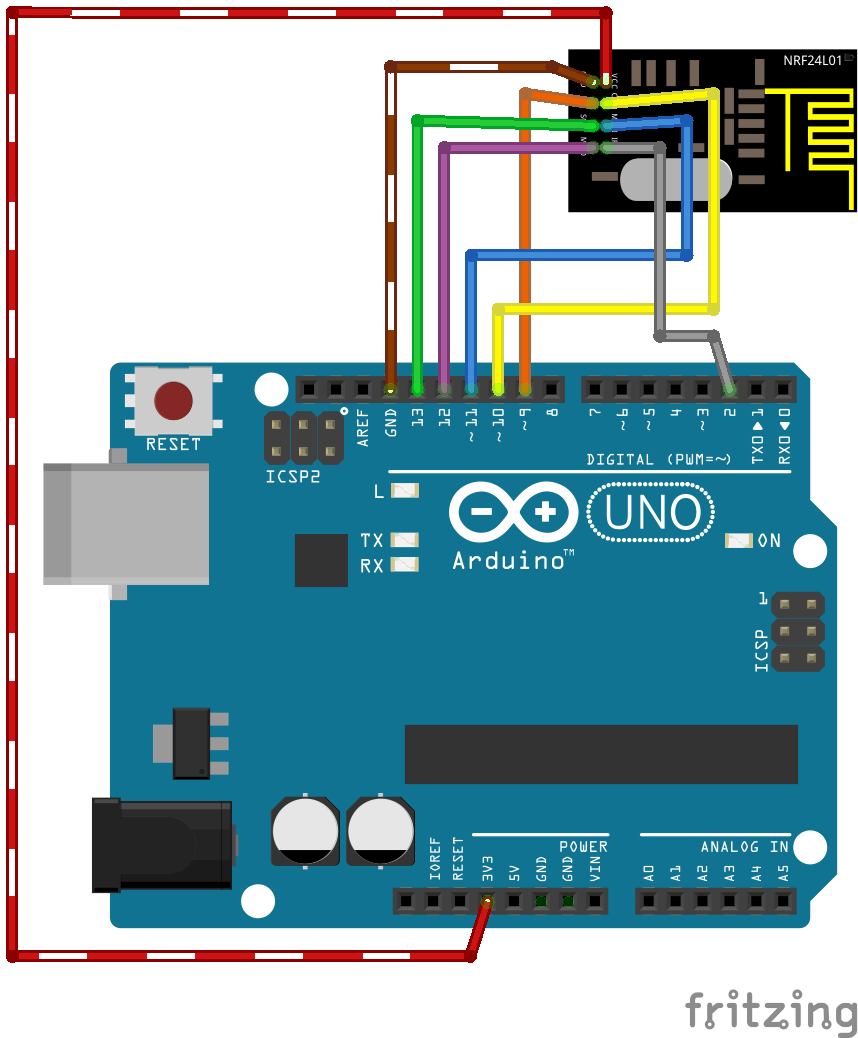
\includegraphics[scale=0.70]{figuras/gateway.png}
      \caption{Gateway}
      \label{fig:gateway2}
\end{figure}
\pagebreak
\vbox{
\indent \rule{10.4cm}{0.6pt}\par
\textbf{Código}\par%\vspace{-0.66\baselineskip}
\rule[0.90\baselineskip]{10.4cm}{0.6pt}
}

\lstinputlisting[language=C++, caption={Gateway}]{code/teste.ino}

\subsection{Nó com sensor DTH11}

\vbox{
\indent \rule{10.4cm}{0.6pt}\par
\textbf{Esquemático}\par%\vspace{-0.66\baselineskip}
\rule[0.90\baselineskip]{10.4cm}{0.6pt}
}

\begin{figure}[ht]
      \centering
      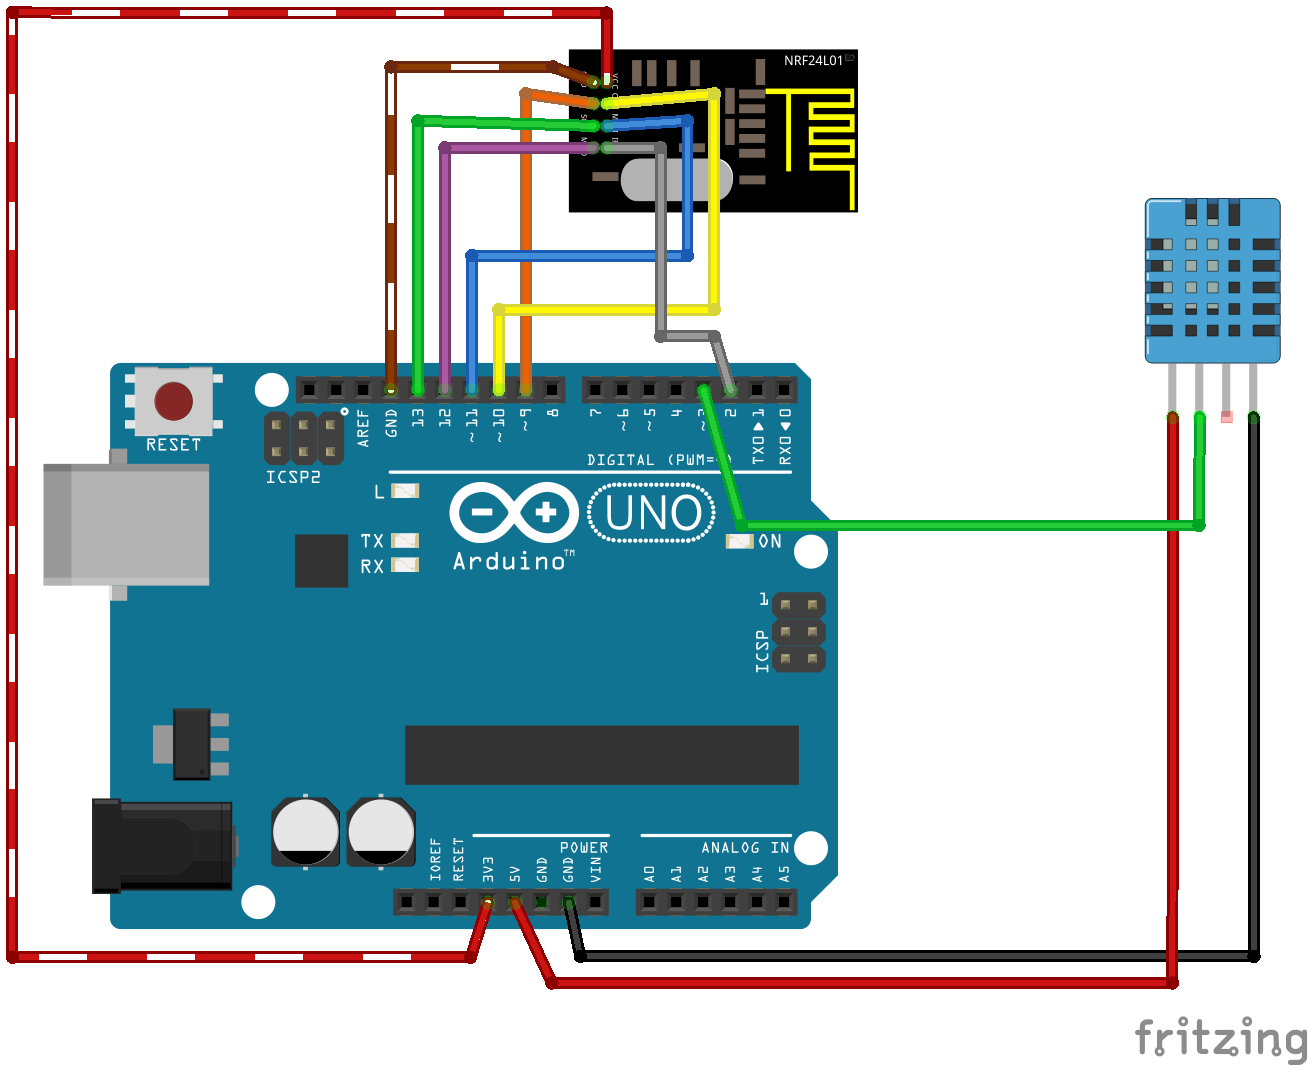
\includegraphics[scale=0.70]{figuras/DTH11_bb.png}
      \caption{Sensor DTH11}
      \label{fig:dth112}
\end{figure}
\pagebreak

\vbox{
\indent \rule{10.4cm}{0.6pt}\par
\textbf{Código}\par%\vspace{-0.66\baselineskip}
\rule[0.90\baselineskip]{10.4cm}{0.6pt}

}

\lstinputlisting[language=C++, caption={DTH11}]{code/dth11.ino}


\subsection{Nó com sensor LDR}

\vbox{
\indent \rule{10.4cm}{0.6pt}\par
\textbf{Esquemático}\par%\vspace{-0.66\baselineskip}
\rule[0.90\baselineskip]{10.4cm}{0.6pt}
}

\begin{figure}[ht]
      \centering
      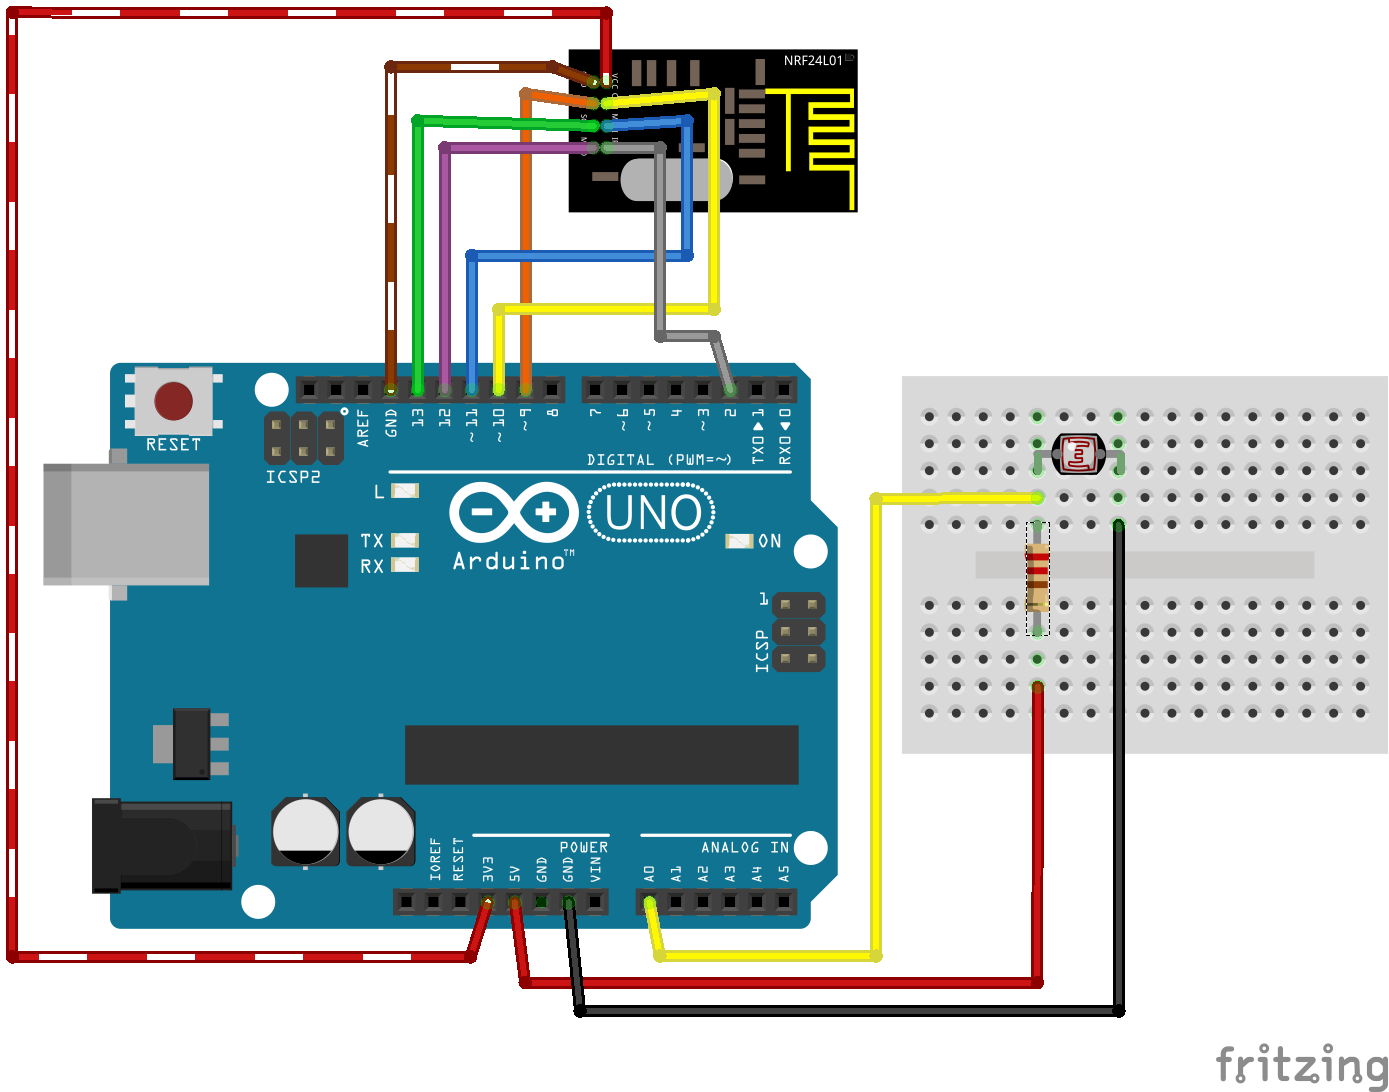
\includegraphics[scale=0.70]{figuras/ldr.png}
      \caption{Sensor LDR}
      \label{fig:ldr2}
\end{figure}
\pagebreak

\vbox{
\indent \rule{10.4cm}{0.6pt}\par
\textbf{Código}\par%\vspace{-0.66\baselineskip}
\rule[0.90\baselineskip]{10.4cm}{0.6pt}

}

\lstinputlisting[language=C++, caption={LDR}]{code/ldr.ino}


\subsection{Controlador}

Arquivo de configuração do Pimatic

\lstinputlisting[language=C++, caption={json.conf}]{code/jsonB.json}
%
\chapter{Projeto C}

Neste projeto, vamos construir uma rede com dois nós. O primeiro nó contém dois sensores e o segundo nó contém um LED atuador. O nó contendo os sensores apresenta dois sensores um DTH11 para coletar informações de temperatura e umidade e um sensor LDR para monitorar a luminosidade do ambiente. Este projeto possui o intuito de apresentar ao leitor o funcionamento de um nó com mais de um sensor e apresentar também um nó atuador. 
Vamos construir um nó sensor para coletar informações de temperatura, umidade e luminosidade e outro nó para emitir um sinal de alerta dependendo das informações dos sensores, os dois nós devem se comunicar com o controlador.

\section{Materiais}

Para esse projeto vamos utilizar os seguintes materiais:
\begin{itemize}
\item 3 Arduinos;
\item Sensor de temperatura e umidade DTH11;
\item Sensor de luminosidade LDR;
\item LED;
\item Resistor 220 ohms;
\item 3 Rádios nRF24L01;
\item Jumpers;
\item Protoboard.
\end{itemize}

Para obter mais informações sobre os materiais consulte o capítulo ~\ref{MateSof}.

\section{Implementação}

\subsection{Gateway}
\vbox{
\indent \rule{10.4cm}{0.6pt}\par
\textbf{Esquemático}\par%\vspace{-0.66\baselineskip}
\rule[0.90\baselineskip]{10.4cm}{0.6pt}
}

\begin{figure}[ht]
      \centering
      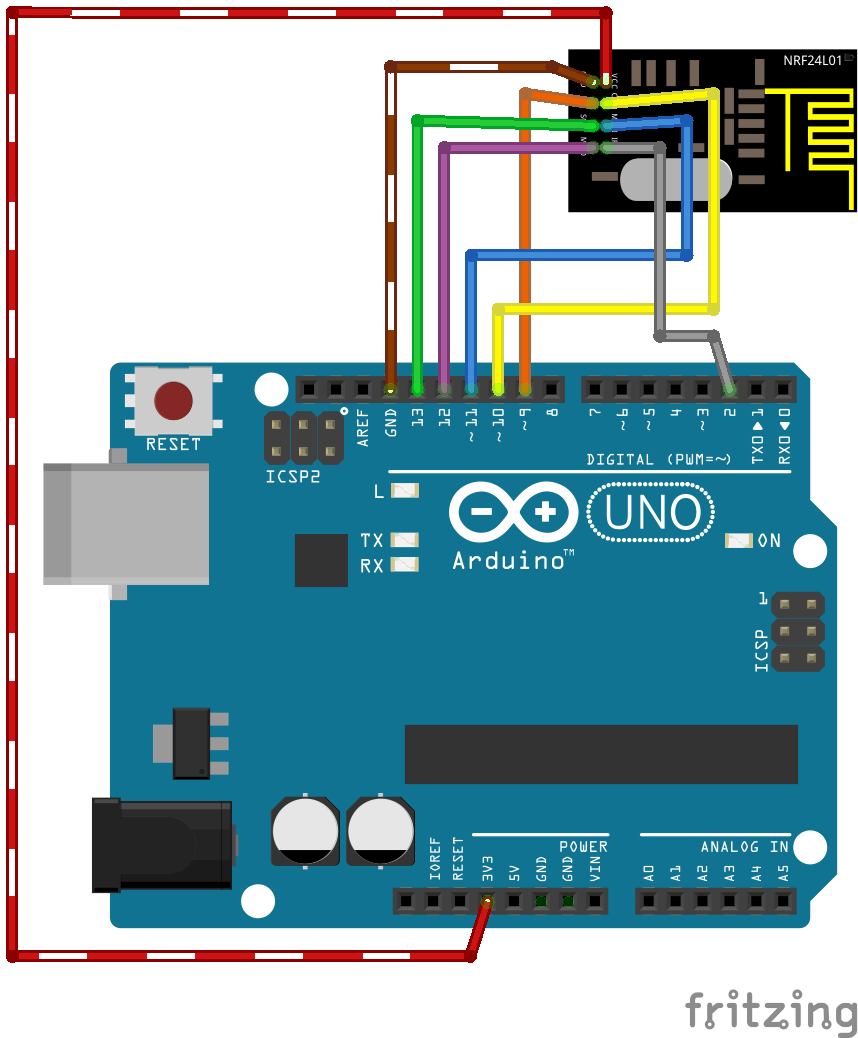
\includegraphics[scale=0.70]{figuras/gateway.png}
      \caption{Gateway}
      \label{fig:gateway3}
\end{figure}
\pagebreak
\vbox{
\indent \rule{10.4cm}{0.6pt}\par
\textbf{Código}\par%\vspace{-0.66\baselineskip}
\rule[0.90\baselineskip]{10.4cm}{0.6pt}
}

\lstinputlisting[language=C++, caption={Gateway}]{code/teste.ino}

\subsection{Nó com sensor DTH11 e LDR}

\vbox{
\indent \rule{10.4cm}{0.6pt}\par
\textbf{Esquemático}\par%\vspace{-0.66\baselineskip}
\rule[0.90\baselineskip]{10.4cm}{0.6pt}
}

\begin{figure}[ht]
      \centering
      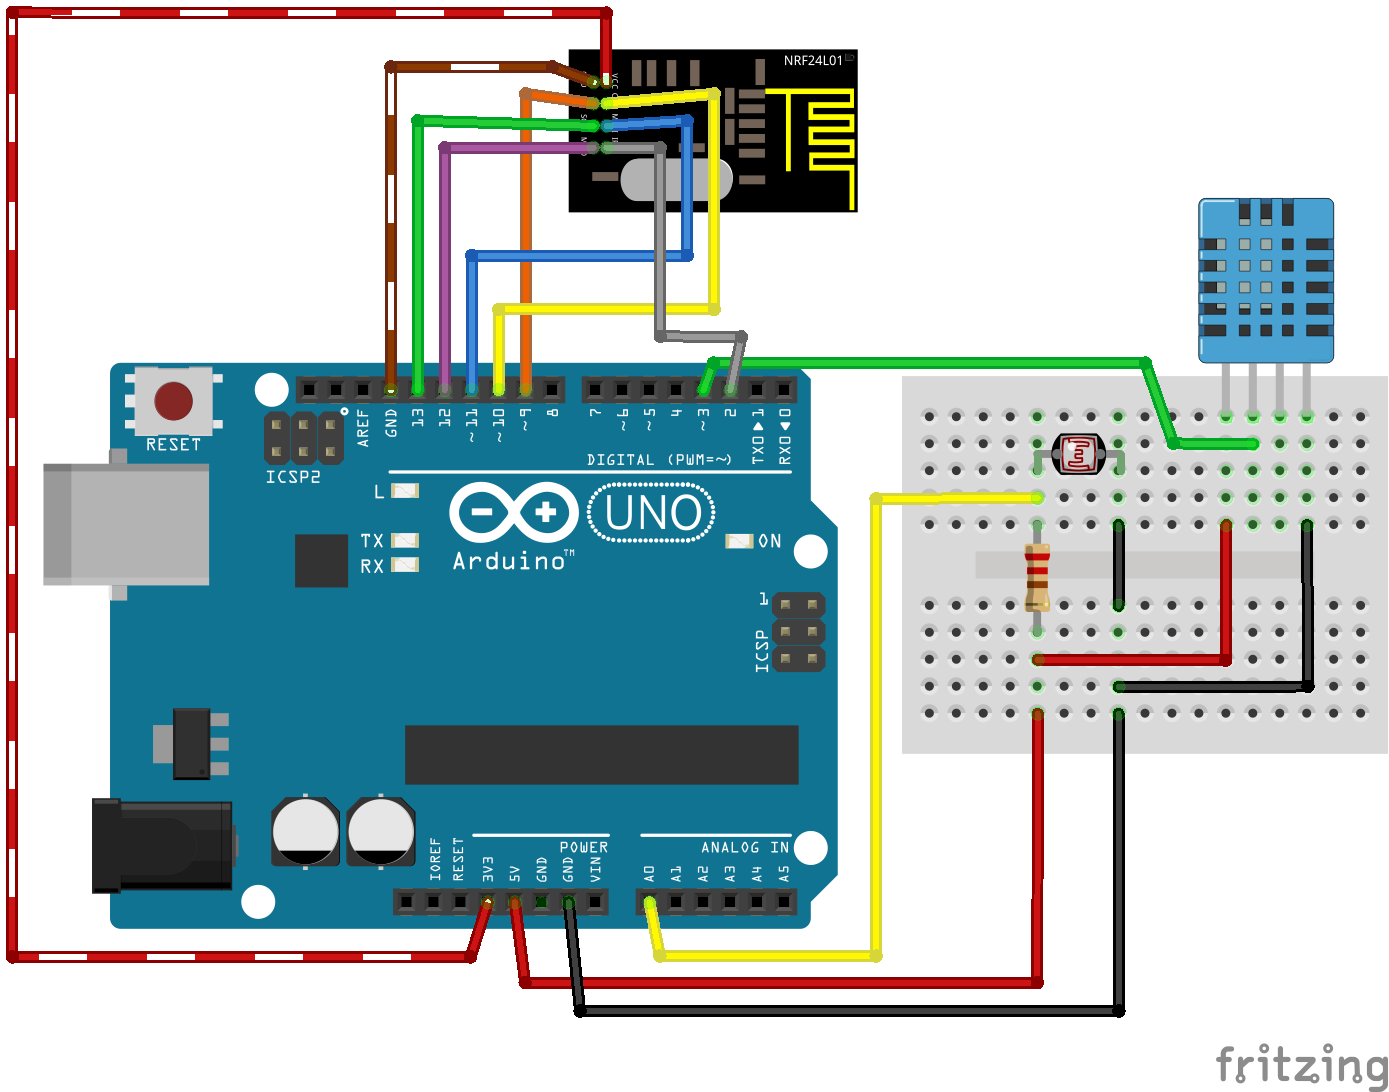
\includegraphics[scale=0.70]{figuras/ldrPdth11_bb.png}
      \caption{Nó Sensor DTH11 e LDR}
      \label{fig:dth11ldr}
\end{figure}
\pagebreak
\vbox{
\indent \rule{10.4cm}{0.6pt}\par
\textbf{Código}\par%\vspace{-0.66\baselineskip}
\rule[0.90\baselineskip]{10.4cm}{0.6pt}
}

\lstinputlisting[language=C++, caption={LDR e DTH11 }]{code/ldr_dth11.ino}


\subsection{Nó com atuador LED}

\vbox{
\indent \rule{10.4cm}{0.6pt}\par
\textbf{Esquemático}\par%\vspace{-0.66\baselineskip}
\rule[0.90\baselineskip]{10.4cm}{0.6pt}
}

\begin{figure}[ht]
      \centering
      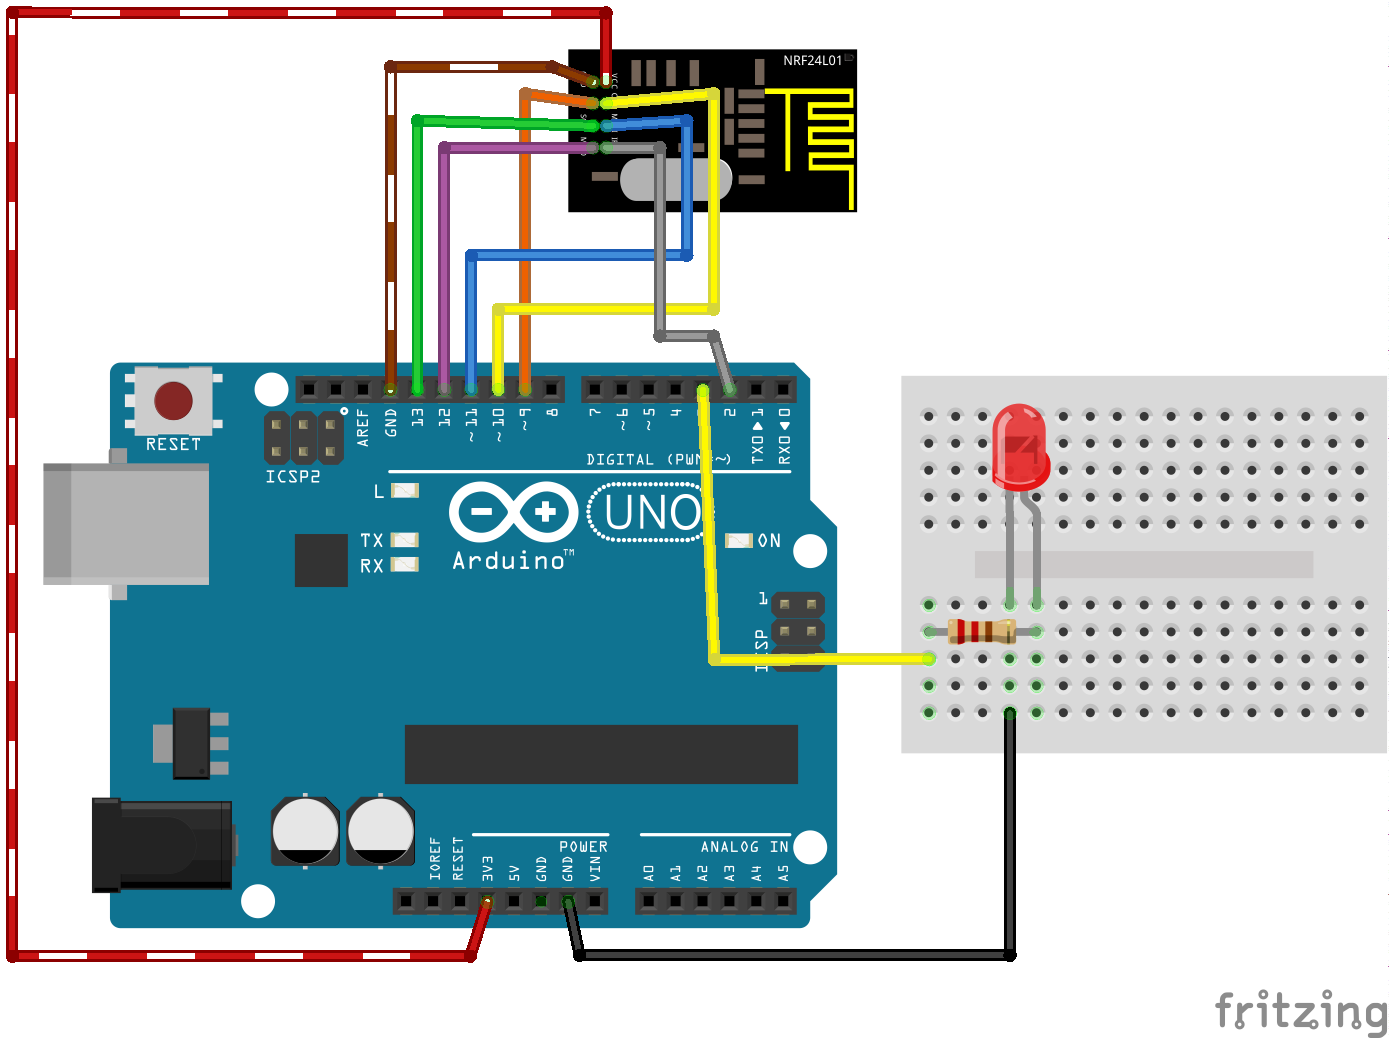
\includegraphics[scale=0.70]{figuras/led_bb.png}
      \caption{Nó LED}
      \label{fig:led}
\end{figure}
\pagebreak
\vbox{
\indent \rule{10.4cm}{0.6pt}\par
\textbf{Código}\par%\vspace{-0.66\baselineskip}
\rule[0.90\baselineskip]{10.4cm}{0.6pt}
}

\lstinputlisting[language=C++, caption={LED}]{code/led.ino}


\subsection{Controlador}

Arquivo de configuração do Pimatic

\lstinputlisting[language=C++, caption={json.conf}]{code/jsonC.json}

%
\backmatter
%

\nocite{faludi2010building}

\bibliographystyle{sbc}
\bibliography{sbc-template}

\end{document}
